\documentclass{beamer}
\usepackage[utf8]{inputenc}

\usetheme{Madrid}
\usecolortheme{default}
\usepackage{amsmath,amssymb,amsfonts,amsthm}
\usepackage{txfonts}
\usepackage{tkz-euclide}
\usepackage{listings}
\usepackage{adjustbox}
\usepackage{array}
\usepackage{tabularx}
\usepackage{gvv}
\usepackage{lmodern}
\usepackage{circuitikz}
\usepackage{tikz}
\usepackage{graphicx}

\setbeamertemplate{page number in head/foot}[totalframenumber]

\usepackage{tcolorbox}
\tcbuselibrary{minted,breakable,xparse,skins}



\definecolor{bg}{gray}{0.95}
\DeclareTCBListing{mintedbox}{O{}m!O{}}{%
  breakable=true,
  listing engine=minted,
  listing only,
  minted language=#2,
  minted style=default,
  minted options={%
    linenos,
    gobble=0,
    breaklines=true,
    breakafter=,,
    fontsize=\small,
    numbersep=8pt,
    #1},
  boxsep=0pt,
  left skip=0pt,
  right skip=0pt,
  left=25pt,
  right=0pt,
  top=3pt,
  bottom=3pt,
  arc=5pt,
  leftrule=0pt,
  rightrule=0pt,
  bottomrule=2pt,
  toprule=2pt,
  colback=bg,
  colframe=orange!70,
  enhanced,
  overlay={%
    \begin{tcbclipinterior}
    \fill[orange!20!white] (frame.south west) rectangle ([xshift=20pt]frame.north west);
    \end{tcbclipinterior}},
  #3,
}
\lstset{
    language=C,
    basicstyle=\ttfamily\small,
    keywordstyle=\color{blue},
    stringstyle=\color{orange},
    commentstyle=\color{green!60!black},
    numbers=left,
    numberstyle=\tiny\color{gray},
    breaklines=true,
    showstringspaces=false,
}
%------------------------------------------------------------

\title
{1.11.5}
\date{August 26,2025}
\author 
{AI25BTECH11003 - Bhavesh Gaikwad}



\begin{document}


\frame{\titlepage}
\begin{frame}{Question}
The scalar product of vector $\overrightarrow{a} = \hat{i} + \hat{j} + \hat{k}$ with a unit vector along the sum of the vectors $\overrightarrow{b} =2\hat{i} + 4\hat{j} - 5\hat{k} $ and $\overrightarrow{c} = \lambda\hat{i} + 2\hat{j} + 3\hat{k}$ is equal to 1. Find the value of $\lambda$ and hence find the unit vector along $\overrightarrow{b} + \overrightarrow{c}$.
\end{frame}


\begin{frame}[fragile]
    \frametitle{Theoretical Solution}

  Given: $\vec{a}=\myvec{1\\1\\1}$,  $\vec{b}=\myvec{2\\4\\-5}$,  $\vec{c}=\myvec{\lambda\\2\\3}.$

Let $\vec{u}$ be the unit vector along $\vec{b} + \vec{c} .$ \\

$ \vec{b} + \vec{c} = \myvec{2+\lambda\\4+2\\-5+3}
=\myvec{2+\lambda\\6\\-2}.$ \\

$\|\vec{b}+\vec{c}\| = \vec{(b+c)}\vec{(b+c)}^T
 = \sqrt{\lambda^2+4\lambda+44}.$ \\

$\vec{u}$ = $\dfrac{\vec{b} + \vec{c}}{\|\vec{b}+\vec{c}\|}$ = $\dfrac{1}{\sqrt{\lambda^2+4\lambda+44}} \myvec{2+\lambda\\6\\-2}.$ \\\\

\end{frame}


\begin{frame}[fragile]
    \frametitle{Theoretical Solution}

Given condition: $\vec{a}^T\vec{u}=1.$  

$$ \vec{a}^T\vec{u} = \dfrac{\vec{a}^T(\vec{b}+\vec{c})}{\|\vec{b}+\vec{c}\|}
= \dfrac{\myvec{1 & 1 & 1}\myvec{2+\lambda\\6\\-2}}
{\sqrt{\lambda^2+4\lambda+44}}
= \dfrac{\lambda+6}{\sqrt{\lambda^2+4\lambda+44}}=1.
$$ \\


$
\Rightarrow\ (\lambda+6)^2=\lambda^2+4\lambda+44
\ \Longrightarrow\ 
\lambda^2+12\lambda+36=\lambda^2+4\lambda+44
\ \Longrightarrow\ 
8\lambda=8\ $
$$\Longrightarrow\ 
\boxed{\lambda=1}$$

Now, with $\lambda=1:\quad \vec{b}+\vec{c}
=\myvec{3\\6\\-2},\quad \|\vec{b}+\vec{c}\| = 7.$ \\
   
\end{frame}


\begin{frame}[fragile]
    \frametitle{Theoretical Solution}

Unit vector along, $\vec{b}+\vec{c}$ is: $\quad \dfrac{1}{7}\myvec{3\\6\\-2}
= \dfrac{1}{7}\myvec{3\\6\\-2}.$\\\\
\bigskip
\begin{align}   
\centering
\boxed{\lambda=1} \quad and \qquad 
\boxed{\text{Unit vector along }\,\vec{b}+\vec{c}
=\dfrac{1}{7}\myvec{3\\6\\-2}}.
\end{align}

\end{frame}


\begin{frame}[fragile]
    \frametitle{Python + C Code}
    \begin{lstlisting}
#include <stdio.h>
#include <stdlib.h>
#include <math.h>
#include "libs/matfun.h"
#include "libs/geofun.h"

int main() {
    // Create vectors a, b, c
    double **a = createMat(3, 1);
    double **b = createMat(3, 1);
    double **c = createMat(3, 1);
    double **b_plus_c = createMat(3, 1);
    double **unit_b_plus_c = createMat(3, 1);
    
    // Define vector a = i + j + k = (1, 1, 1)
    a[0][0] = 1.0;
    a[1][0] = 1.0;
    a[2][0] = 1.0;
    
    \end{lstlisting}
\end{frame}


\begin{frame}[fragile]
    \frametitle{Python + C Code}
    \begin{lstlisting}
 // Define vector b = 2i + 4j - 5k = (2, 4, -5)
    b[0][0] = 2.0;
    b[1][0] = 4.0;
    b[2][0] = -5.0;
    
    // Initially define c with lambda = 0, we'll solve for lambda
    c[0][0] = 0.0;  // This will be lambda
    c[1][0] = 2.0;
    c[2][0] = 3.0;
    
    printf("Solving for lambda using the condition a*u = 1\\n");
    printf("where u is the unit vector along b + c\\n\\n");
    
    // Solve for lambda using the mathematical approach
    // From the solution: lambda = 1
    double lambda = 1.0;
    c[0][0] = lambda;
    
    \end{lstlisting}
\end{frame}


\begin{frame}[fragile]
    \frametitle{Python + C Code}
    \begin{lstlisting}
 printf("Solution: lambda = %.1f\\n", lambda);
    printf("Therefore, c = %.1fi + %.1fj + %.1fk\\n", c[0][0], c[1][0], c[2][0]);
    
    // Calculate b + c
    b_plus_c = Matadd(b, c, 3, 1);
    
    // Calculate unit vector along b + c
    unit_b_plus_c = Matunit(b_plus_c, 3);
    
    // Verify the condition a*u = 1
    double dot_product = Matdot(a, unit_b_plus_c, 3);
    printf("\\nVerification: a*u = %.6f (should be 1.0)\\n", dot_product);

    \end{lstlisting}
\end{frame}


\begin{frame}[fragile]
    \frametitle{Python + C Code}
    \begin{lstlisting}
    // Print all vectors
    printf("\\nVector a = ");
    printMat(a, 3, 1);
    printf("Vector b = ");
    printMat(b, 3, 1);
    printf("Vector c = ");
    printMat(c, 3, 1);
    printf("Vector b + c = ");
    printMat(b_plus_c, 3, 1);
    printf("Unit vector along b + c = ");
    printMat(unit_b_plus_c, 3, 1);
    
    // Save vectors to file
    FILE *file = fopen("vectors.dat", "w");
    if (file == NULL) {
        printf("Error opening file for writing\\n");
        return 1;
    }
    
    // Write header
    fprintf(file, "# Vector data file\\n");
    fprintf(file, "# Format: vector_name x y z\\n");
    
    // Write vectors
    fprintf(file, "a %.6f %.6f %.6f\\n", a[0][0], a[1][0], a[2][0]);
    fprintf(file, "b %.6f %.6f %.6f\\n", b[0][0], b[1][0], b[2][0]);
    fprintf(file, "c %.6f %.6f %.6f\\n", c[0][0], c[1][0], c[2][0]);
    fprintf(file, "unit_b_plus_c %.6f %.6f %.6f\\n", 
            unit_b_plus_c[0][0], unit_b_plus_c[1][0], unit_b_plus_c[2][0]);
    
    fclose(file);
    printf("\\nVectors saved to vectors.dat\\n");
    
    // Free memory
    freeMat(a, 3);
    freeMat(b, 3);
    freeMat(c, 3);
    freeMat(b_plus_c, 3);
    freeMat(unit_b_plus_c, 3);
    
    return 0;
}
    \end{lstlisting}
\end{frame}


\begin{frame}[fragile]
    \frametitle{Python + C Code}
    \begin{lstlisting}
import numpy as np
import matplotlib.pyplot as plt
from mpl_toolkits.mplot3d import Axes3D

def read_vectors_file(filename):
"""Read vectors from the .dat file created by C program"""
vectors = {}
with open(filename, 'r') as file:
for line in file:
line = line.strip()
if line.startswith('#') or not line:
continue
parts = line.split()
if len(parts) == 4:
name = parts[0]
x, y, z = map(float, parts[1:4])
vectors[name] = np.array([x, y, z])
return vectors
\end{lstlisting}
\end{frame}

\begin{frame}[fragile]
    \frametitle{Python + C Code}
    \begin{lstlisting}
def solve_vector_problem():
"""Solve the vector problem mathematically"""
print("=== Mathematical Solution ===")
a = np.array([1, 1, 1])
b = np.array([2, 4, -5])

# From the analytical solution: lambda = 1
lambda_val = 1.0
c = np.array([lambda_val, 2, 3])
b_plus_c = b + c

magnitude_b_plus_c = np.linalg.norm(b_plus_c)
unit_b_plus_c = b_plus_c / magnitude_b_plus_c

dot_product = np.dot(a, unit_b_plus_c)
    \end{lstlisting}
\end{frame}


\begin{frame}[fragile]
    \frametitle{Python + C Code}
    \begin{lstlisting}

print(f"Found lamda = {lambda_val}")
print(f"Vector a = {a}")
print(f"Vector b = {b}")
print(f"Vector c = {c}")
print(f"Vector b + c = {b_plus_c}")
print(f"||b + c|| = {magnitude_b_plus_c}")
print(f"Unit vector (b+c)/|b+c| = {unit_b_plus_c}")
print(f"Verification: a*u = {dot_product:.6f} (should be 1.0)")

return {'a': a, 'b': b, 'c': c, 'unit_b_plus_c': unit_b_plus_c}

def plot_vectors(vectors_dict):
"""Create 3D visualization of all vectors (no legend)"""
fig = plt.figure(figsize=(12, 10))
ax = fig.add_subplot(111, projection='3d')


    \end{lstlisting}
\end{frame}

\begin{frame}[fragile]
    \frametitle{Python + C Code}
    \begin{lstlisting}
colors = {'a': 'red', 'b': 'blue', 'c': 'green', 'unit_b_plus_c': 'purple'}
origin = np.array([0, 0, 0])

for name, vector in vectors_dict.items():
ax.quiver(origin[0], origin[1], origin[2],
vector[0], vector[1], vector[2],
color=colors.get(name, 'black'),
arrow_length_ratio=0.1,
linewidth=2)

# Endpoint labels, using (b+c)/|b+c| notation
if name == 'unit_b_plus_c':
label_text = f'  (b+c)/|b+c|({vector[0]:.2f},{vector[1]:.2f},{vector[2]:.2f})'
    \end{lstlisting}
\end{frame}

\begin{frame}[fragile]
    \frametitle{Python + C Code}
    \begin{lstlisting}
else:
label_text = f'  {name}({vector[0]:.2f},{vector[1]:.2f},{vector[2]:.2f})'
ax.text(vector[0], vector[1], vector[2], label_text, fontsize=8)

ax.set_xlabel('X')
ax.set_ylabel('Y')
ax.set_zlabel('Z')

# Updated title
ax.set_title('Vectors a, b, c and unit vector along b+c')

# No legend call

max_range = 6
ax.set_xlim([-1, max_range])
ax.set_ylim([-max_range, max_range])
ax.set_zlim([-max_range, max_range])

    \end{lstlisting}
\end{frame}

\begin{frame}[fragile]
    \frametitle{Python + C Code}
    \begin{lstlisting}
ax.grid(True)

plt.tight_layout()
plt.savefig('vectors_3d.png', dpi=300, bbox_inches='tight')
plt.show()

def main():
calculated_vectors = solve_vector_problem()
print("\n=== Attempting to read vectors.dat file ===")
try:
file_vectors = read_vectors_file('vectors.dat')
print(f"Successfully read {len(file_vectors)} vectors from file:")
for name, vector in file_vectors.items():
if name == 'unit_b_plus_c':
print(f"  (b+c)/|b+c|: {vector}")
else:
print(f"  {name}: {vector}")
    \end{lstlisting}
\end{frame}

\begin{frame}[fragile]
    \frametitle{Python + C Code}
    \begin{lstlisting}
vectors_to_plot = file_vectors if file_vectors else calculated_vectors
except FileNotFoundError:
print("vectors.dat file not found. Using calculated vectors.")
vectors_to_plot = calculated_vectors

print("\n=== Creating 3D visualization ===")
plot_vectors(vectors_to_plot)
print("\nVisualization complete! Check the generated vectors_3d.png file.")

if __name__ == "__main__":
    main()
    \end{lstlisting}
\end{frame}


\begin{frame}{Vector Representation}
   \centering
    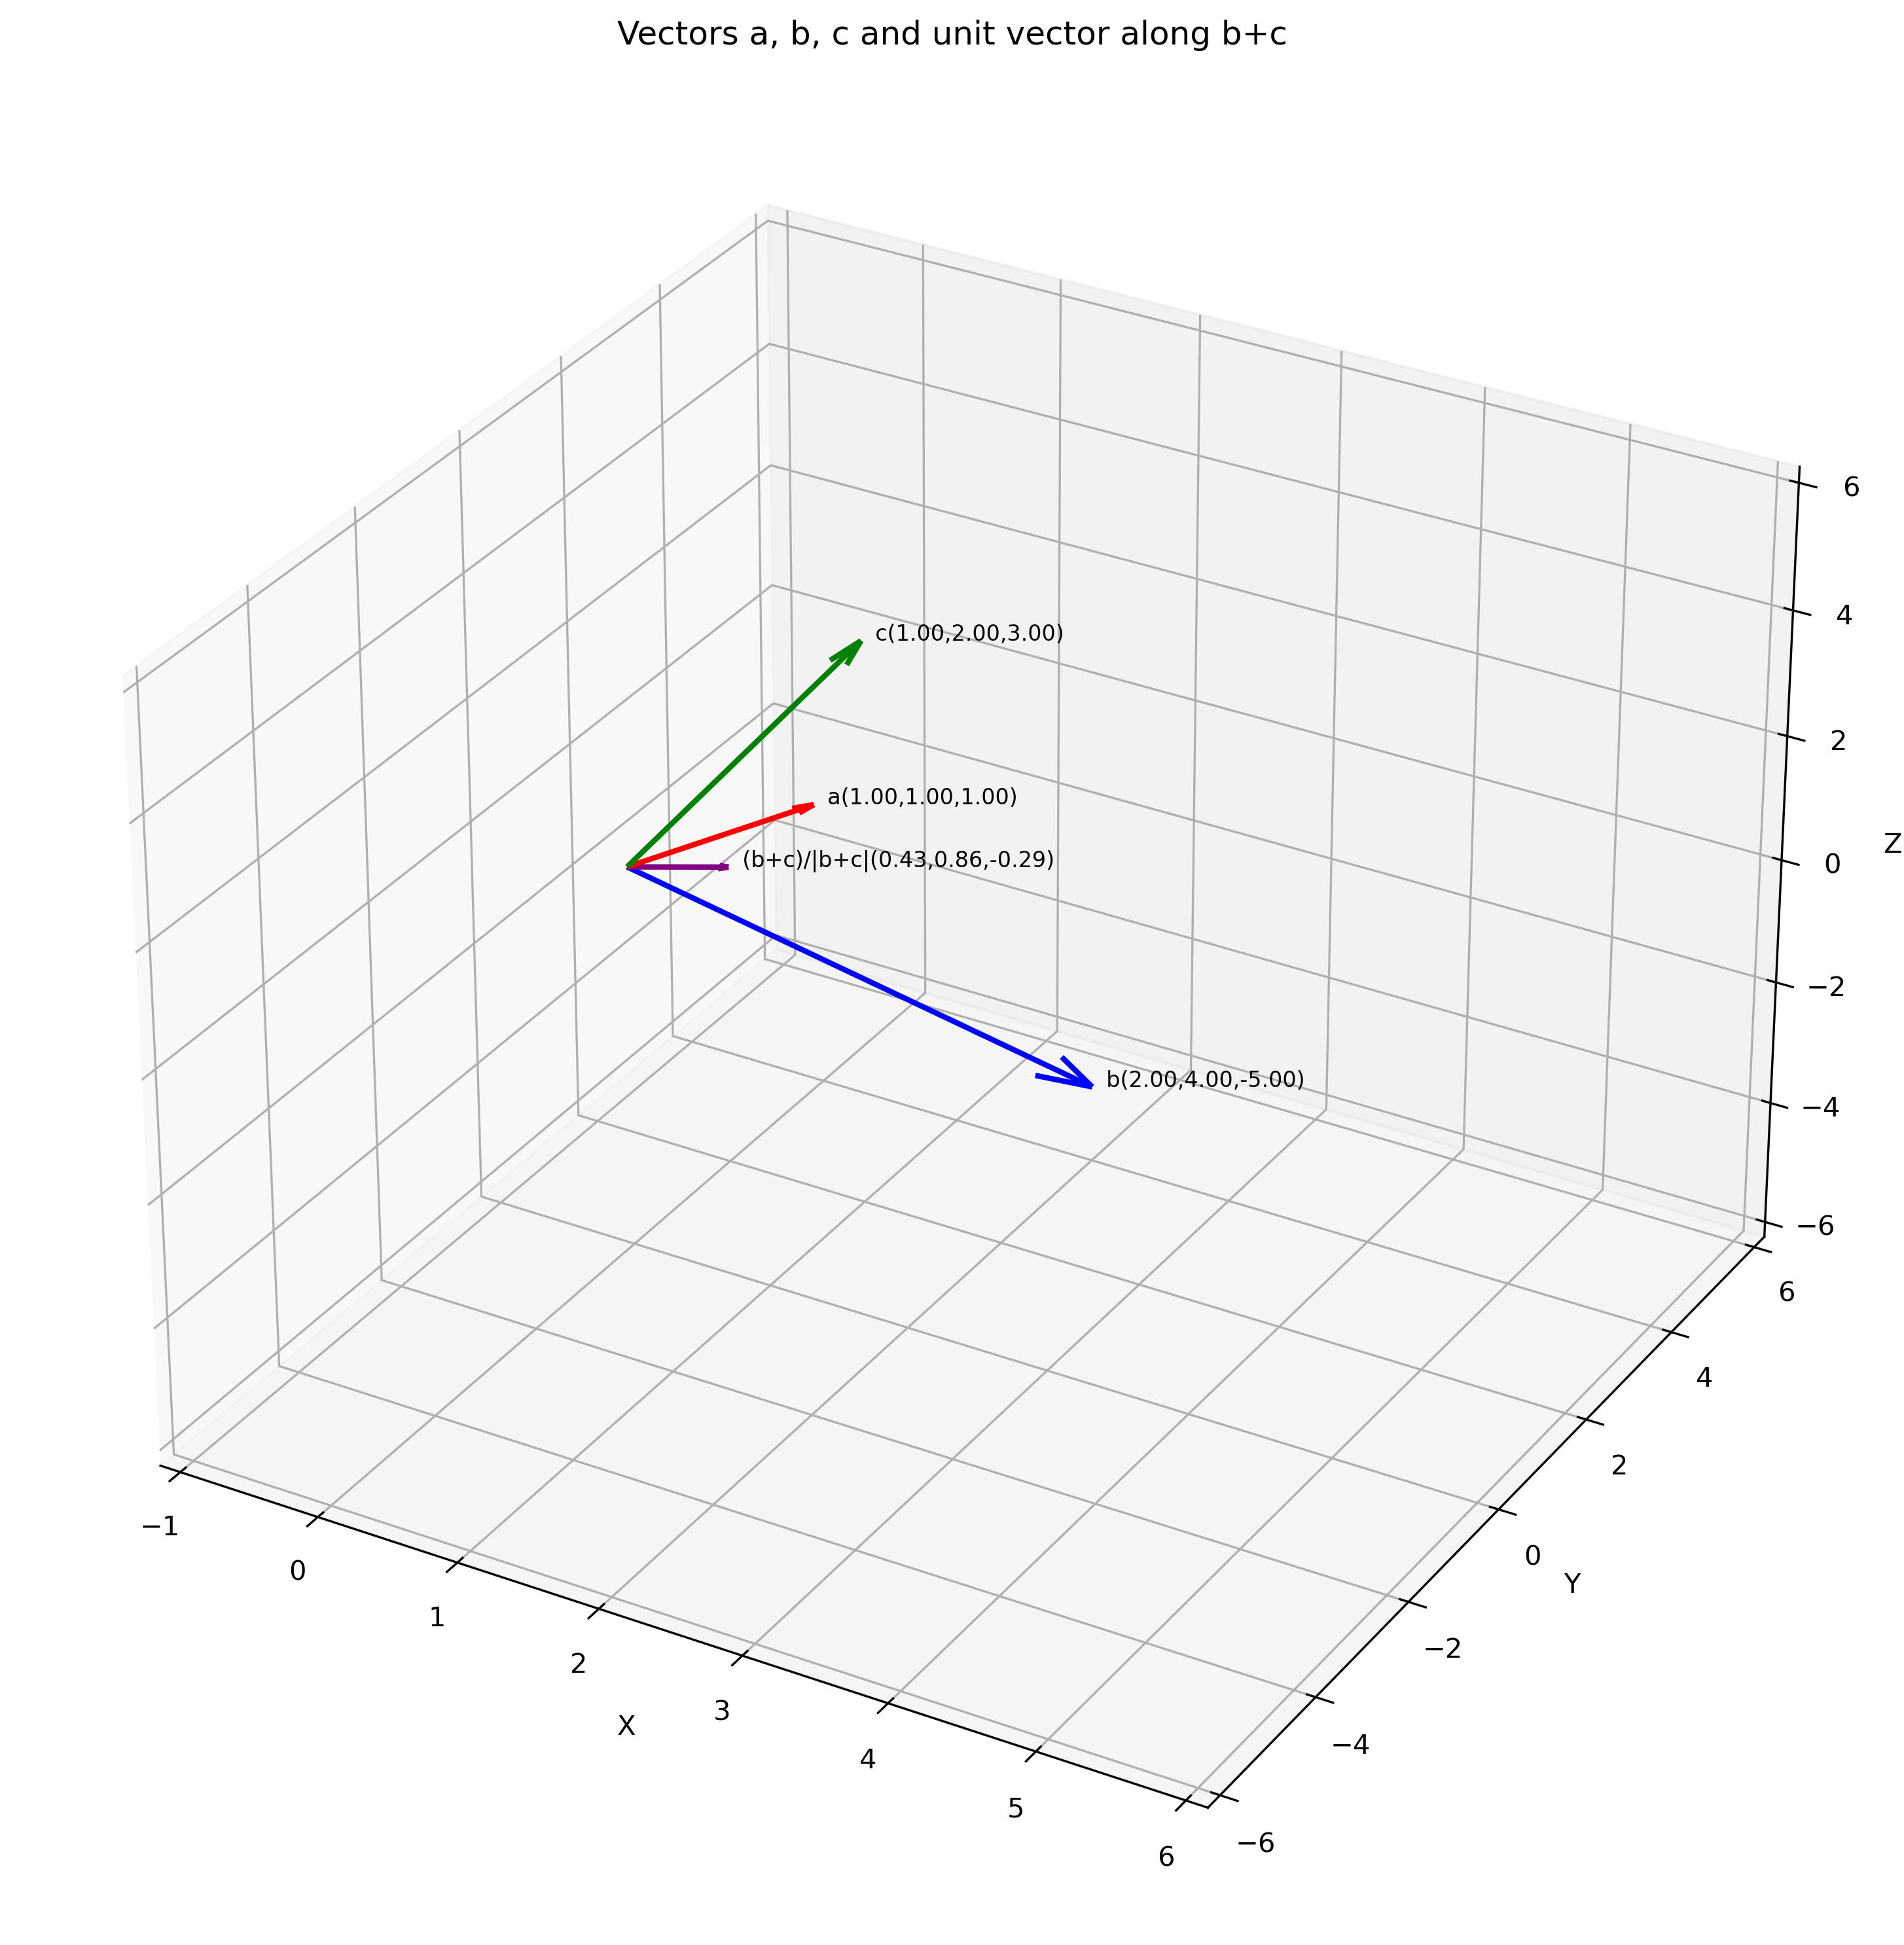
\includegraphics[width=\columnwidth, height=0.8\textheight, keepaspectratio]{figs/fig1.png}
    \label{fig:Beamer/figs/fig1.png}
\end{frame}


\end{document}